\chapter{Introduction} \label{chp:introduction}

\section{Motivation}

\acrfullpl{dcc}---also known as cumulonimbus (\textit{`heaped raincloud'}) or thunderstorms---are dynamical atmospheric phenomena resulting from instability in the troposphere.
\acrshort{dcc}s consist of tall, central `cores' surrounded by a large, detrained cirrus `anvil' (see fig.~\ref{fig:cb_photo}).
The central cores of \acrshort{dcc}s form around intense convective updrafts that transport water from near the surface to the upper troposphere.
At the top of these updrafts, the divergence of the cloudy airmass leads to the formation of a large area of detrained anvil that extends beyond the footprint of the core.
With heights exceeding 10\,\unit{km}, and anvils that measure hundreds or thousands of km in extent, \acrshort{dcc}s form some of the most physically imposing objects in the atmosphere, and have important impacts on weather and climate.

\begin{figure}[tp]
    \centering
    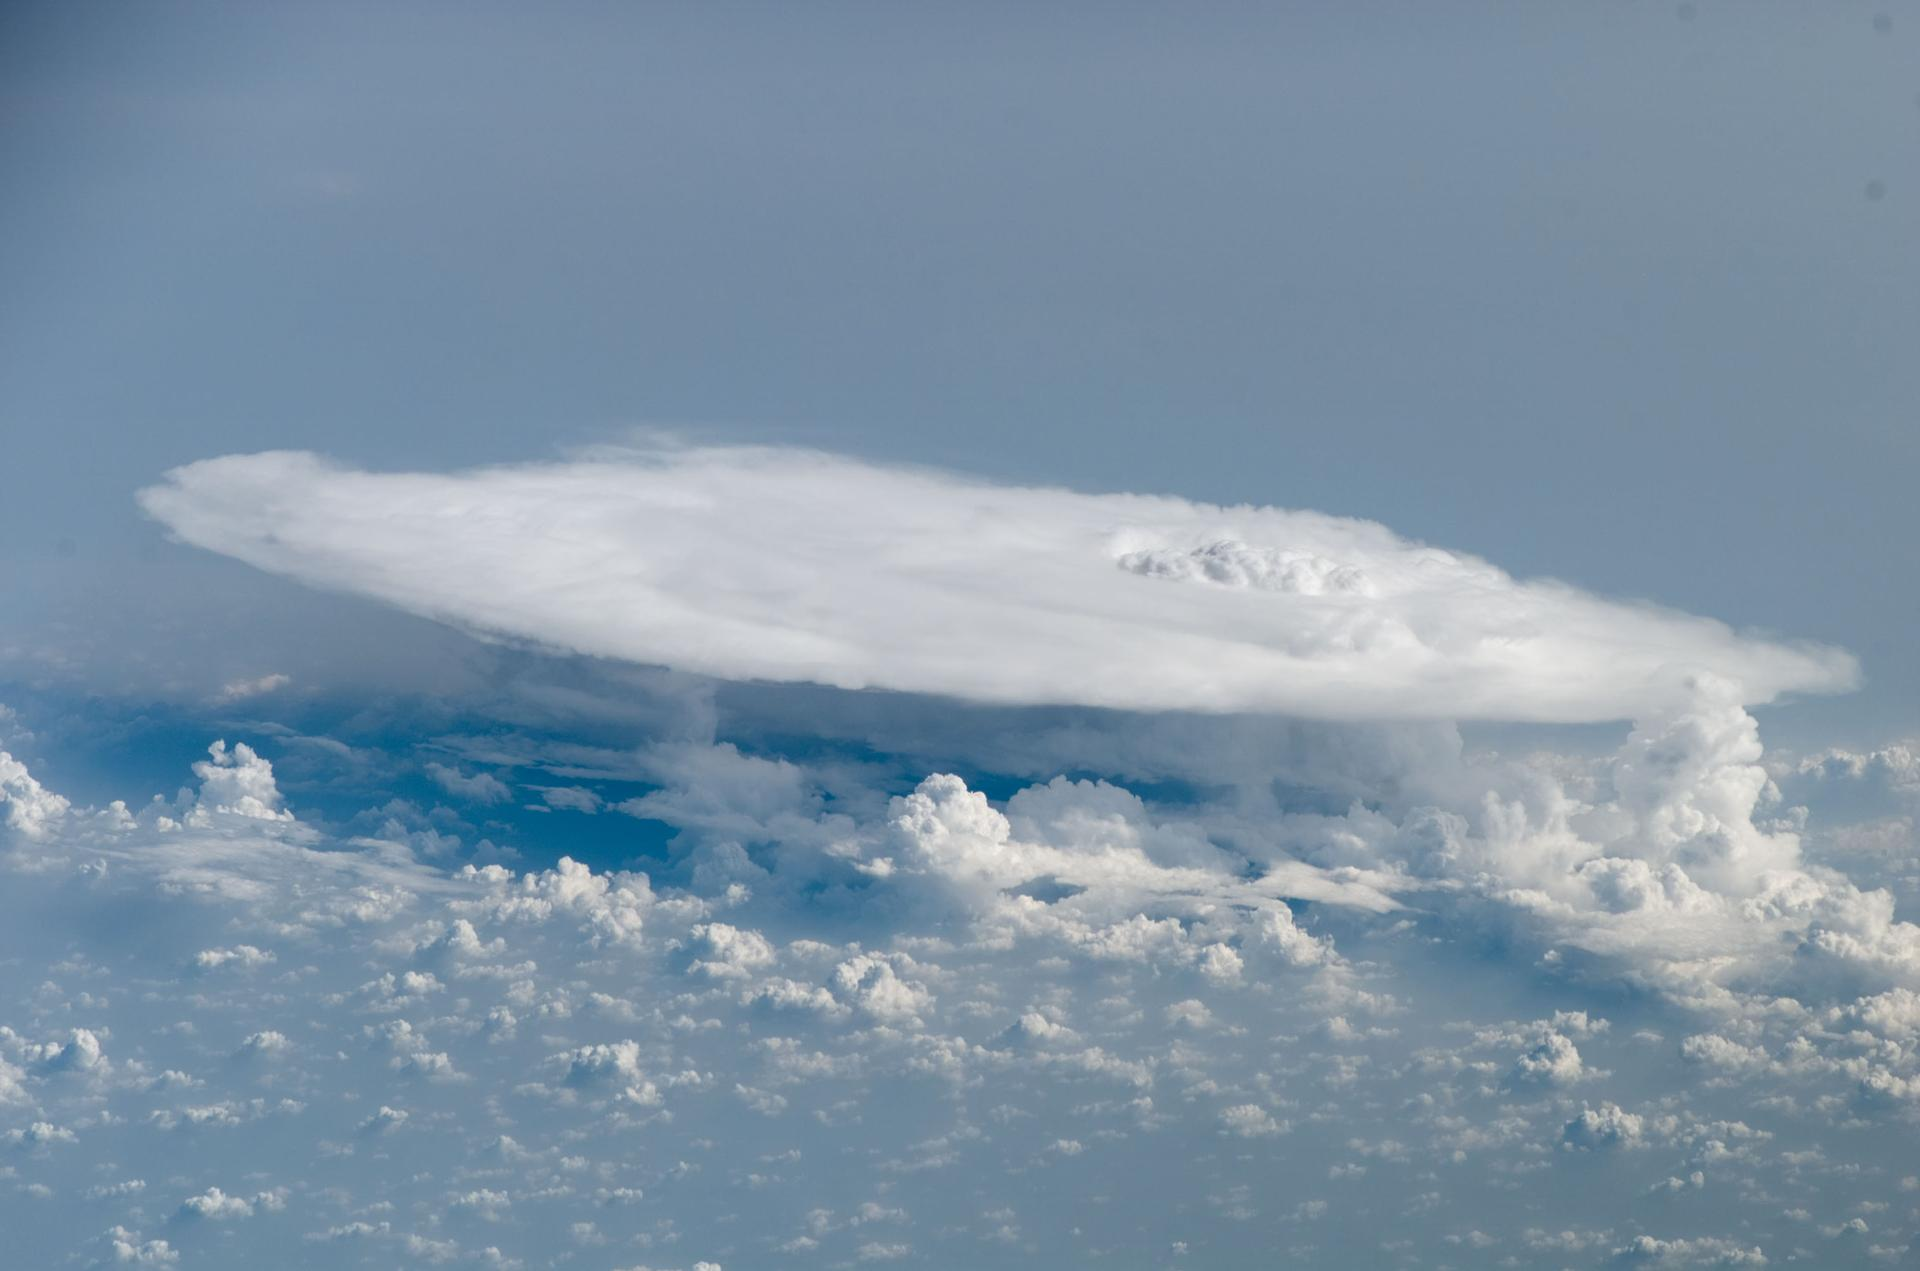
\includegraphics[width=\textwidth]{figures/cumulonimbus_nasa.jpg}
    \caption[
    A photograph of a \acrshort{dcc} seen over Africa from the ISS
    ]{
    A photograph of a \acrshort{dcc} seen over Africa from the International Space Station on 5th February 2008. The main convective core can be seen in the centre of the image as the turbulent, textured region emerging through the wide, flat anvil that surrounds it. On the right-hand side of the image a new core can be seen developing that is about to make contact with the anvil of the original core. Image credit: \acrshort{nasa} Image and Video Library, iss016e027426.
    }
    \label{fig:cb_photo}
\end{figure}

First identified as a unique cloud type in the late 19\textsuperscript{th}~century by \citet{abercromby_identity_1887} and \citet{hildebrandsson_remarks_1887}, \acrshort{dcc}s have been a focus of scientific investigation ever since.
\acrshort{dcc}s are the source of many severe weather events \citep{matsudo_severe_2011, houze_chapter_2014} including heavy precipitation \citep{westra_future_2014}, lightning \citep{williams_radar_1992}, hail \citep{punge_hail_2016}, flooding, tornadoes and tropical cyclones.

\acrshort{dcc}s play an important role in weather and climate beyond extreme events.
In the tropics, deep convection forms the ascending branch of the Hadley cell \citep{riehl_heat_1958}, and in doing so begins the transport of energy through the atmosphere from the equator to the poles.
In many regions of the world, from tropical Africa to the Great Plains of North America, \acrshort{dcc}s provide the majority of precipitation \citep{feng_global_2021}.
The large anvil clouds of \acrshort{dcc}s have a mediating effect on the radiative heating of the climate, reflecting incoming sunlight and trapping outgoing longwave radiation in equal amounts \citep{ramanathan_cloud-radiative_1989, hartmann_effect_1992, hartmann_tropical_2016}.

\acrshort{dcc}s are expected to have multiple responses to climate change.
Increases in atmospheric temperature and humidity increase both the intensity and frequency of heavy precipitation from deep convection \citep[e.g.][]{allen_constraints_2002, trenberth_changing_2003, held_robust_2006}.
In addition, global warming is also expected to lead to multiple radiative feedbacks from convective anvil clouds with both positive (warming) and negative (cooling) impacts \citep{bony_clouds_2015}.
These feedbacks remain one of the largest uncertainties in future climate projections \citep{sherwood_assessment_2020}.
Understanding the behaviour, interactions and feedbacks of \acrshort{dcc}s is therefore vital for understanding both our present-day climate and its response in a changing world \citep{gasparini_opinion_2023}.

Anthropogenic aerosols also affect \acrshort{dcc}s through aerosol--cloud interactions such as convective invigoration \citep{khain2005aerosol, rosenfeld_flood_2008}, although these processes remain uncertain \citep{varble_opinion_2023}.
Aerosol impacts on \acrshort{dcc}s are difficult to study in observations due to the small magnitude of the effects in comparison to meteorological variability and measurement uncertainty \citep{grabowski_can_2018}, as well as the difficulty in separating aerosol--cloud interactions from confounding processes \citep{varble_erroneous_2018}.
As a result, the effects of aerosols on \acrshort{dcc}s are not considered within the scope of this thesis.

\acrshort{dcc}s occur over a wide range of scales, and this limits the sources of observations which can fully capture their behaviour.
The processes of individual \acrshort{dcc}s span a scale from single kilometres and minutes, to hundreds of km and multiple days for large, organised convective systems.
When considering the response of the global circulation and atmospheric energy balance, it may take multiple years of observations for an equilibrium state to be observed \citep{muller_energetic_2011}.
Geostationary weather satellites, such as the \acrfull{noaa} \acrfull{goes} series and the \acrfull{eumetsat} Meteosat series have provided imagery of \acrshort{dcc}s over many decades for the purpose of monitoring and predicting the weather.
However, these instruments have not traditionally supported the accuracy required for scientific studies, and it is only with the latest generation that the capability of this imagery for studying the behaviour of deep convection is being fully realised.

The study of \acrshort{dcc}s is made difficult by their complex, dynamic behaviours.
Many techniques used to study more slowly varying or spatially uniform atmospheric phenomena (including other cloud types, such as stratus and cumulostratus regions) cannot fully capture the complexity of \acrshort{dcc}s.
Even snapshot observations, such as those made by polar-orbiting earth observation satellites, cannot fully characterise \acrshort{dcc} behaviour, no matter how detailed they are, due to the rapid changes in the properties of \acrshort{dcc}s over their lifetimes.
Lagrangian methods---those which follow the \acrshort{dcc}s' motion---provide vital observations of \acrshort{dcc} properties over their lifecycle.
While particle trajectory models have been successfully utilised to study boundary layer clouds from a Lagrangian perspective \citep[e.g][]{eastman_competing_2018, christensen_aerosols_2020a}, these techniques are not easily applicable due to the complex wind environment of \acrshort{dcc}s, and the low accuracy of reanalysis models and derived \acrfullpl{amv} in these environments.
Instead, image processing methods that detect and track \acrshort{dcc}s are used to study their behaviour from a Lagrangian perspective.
These methods have seen a renaissance in recent years for studying deep convection, with applications including convective resolving models, weather radars and geostationary satellite imagery.
There remain a number of limitations in existing tracking models, and so the development of novel techniques is required to better understand the full spectrum of \acrshort{dcc}s.

Overall, understanding the behaviour of \acrshort{dcc}s and their response to climate change is vital both to predicting extreme weather events and climate feedbacks.
This introductory chapter will explore a range of topics regarding the behaviour of \acrshort{dcc}s and their further impacts.
In particular, it will focus on the relation between deep convection and the behaviour of anvil clouds, and how novel cloud tracking methods can be used to provide new insights from observations of \acrshort{dcc}s.


\section{Physical properties of \acrshort{dcc}s}

The physical nature of a \acrshort{dcc} can be divided into three parts: a cloud system, consisting of a multitude of liquid and ice water cloud particles along with several kinds of precipitation; a thermodynamic system in which moisture and energy are transformed into intense vertical motion and circulations across several scales; and a radiative system in which the large anvil reflects sunlight and absorbs \acrshort{lw} radiation, both heating and cooling the atmosphere within and below it.
These processes are not independent and interact with each other in numerous ways.
As a result, understanding each of them is important to understanding the behaviour of \acrshort{dcc}s.


\subsection{Cloud microphysical properties}

\acrshort{dcc}s, like any other cloud, are formed from a great number of water and ice particles suspended in the atmosphere.
\acrshort{dcc}s consist of a vertically growing core spanning from the \acrfull{pbl} to the tropopause, a distance often exceeding 10\,\unit{km}, with a diameter of ~10\,\unit{km} and updraught velocities of around 10\,\unit{ms\textsuperscript{-1}} \citep{weisman_mesoscale_2015}, and a surrounding anvil cloud formed due to horizontal divergence of cloud ice which has been lifted to the level of neutral buoyancy \citep{houze_chapter_2014}.
While the anvil cirrus of a \acrshort{dcc} consists of ice particles, many of these particles form in the liquid phase within the core, before freezing as they are lifted vertically and then detrained horizontally.
As a result, while ice--phase microphysics determines the evolution of anvil cirrus over time, liquid--phase microphysics are also important in \acrshort{dcc}s due to the initial formation of many anvil particles by homogeneous freezing of liquid droplets formed in the convective core.

% \begin{equation}
%     \frac{1}{e_s}\frac{d e_s}{dT} \cong \frac{L}{R_v T^2}
%     % \caption{The Clausius--Clapeyron relation for saturation vapour pressure}
% \end{equation}

\begin{eqfloat}
    \captionsetup{labelformat=empty}
    \caption{
    The Clausius--Clapeyron relation for saturation vapour pressure (eq.~\ref{eq:cc_rel}), where $e_s$ is the saturation vapour pressure, $T$ is the parcel temperature in Kelvin, $L_\mathrm{v}(T, p)$ is the latent heat of vaporisation of water, and $R_\mathrm{v}$ is the gas constant of water vapour. This cannot be solved analytically due to the temperature dependence of the latent heat of vaporisation. An accurate approximation in the form of the August--Roche--Magnus equation \citep{magnus_versuche_1844} be found empirically (eq.~\ref{eq:cc_rel_approx}, with coefficients from \citet{alduchov_improved_1997}).
    Similarly, the relation for saturation vapour pressure over ice ($e_\mathrm{s,i}$) is given by eq.~\ref{eq:cc_ice_rel}, where $L_\mathrm{s}(T,P)$ is the latent heat of sublimation of water (equivalent to $L_\mathrm{v} + L_\mathrm{f}$, the latent heat of fusion). 
    The empirical approximation for $e_\mathrm{s,i}$ is given by eq.~\ref{eq:cc_ice_rel_approx}.
    Note that at 0\,\textdegree C, $e_\mathrm{s,i} = e_\mathrm{s}$, whereas the the approximations differ slightly.
    }
    
    \begin{equation} 
    \label{eq:cc_rel}
        \frac{1}{e_{\mathrm{s}}}\frac{\mathrm{d} e_{\mathrm{s}}}{\mathrm{d} T} = \frac{L_\mathrm{v}(T, p)}{R_\mathrm{v} T^2}
    \end{equation}
    
    \begin{equation}
    \label{eq:cc_rel_approx}
        e_\mathrm{s}\left ( T \right ) \cong 6.1094\ \mathrm{kPa} \left ( \frac{17.625\ \mathrm{K}^{-1} \cdot (T - 273.15\ \mathrm{K})}{T - 30.11\ \mathrm{K}} \right )
    \end{equation}

    \begin{equation} 
    \label{eq:cc_ice_rel}
        \frac{1}{e_\mathrm{s,i}}\frac{\mathrm{d} e_{\mathrm{s,i}}}{\mathrm{d} T} = \frac{L_\mathrm{s}(T, p)}{R_\mathrm{v} T^2}
    \end{equation}
    
    \begin{equation}
    \label{eq:cc_ice_rel_approx}
        e_\mathrm{s,i}\left ( T \right ) \cong 6.1121\ \mathrm{kPa} \left ( \frac{22.587\ \mathrm{K}^{-1} \cdot (T - 273.15\ \mathrm{K})}{T + 0.71\ \mathrm{K}} \right )
    \end{equation}
    
\end{eqfloat}

When an airmass containing water vapour is lifted it expands and cools.
In doing so, the saturation vapour pressure decreases---in accordance with the Clausius-Clapeyron relation (eq.~\ref{eq:cc_rel})---at a faster rate than the specific vapour pressure of the airmass.
When the vapour pressure of the airmass exceeds the saturation vapour pressure it is considered supersaturated, and can condense to form cloud droplets.
It is very difficult for water droplets to form in a perfectly clean atmosphere, since for this to happen supersaturation of several hundred percent would be required.
Instead, soluble aerosol particles in the supersaturated airmass become the surface on which cloud droplets form, a process known as \acrfull{ccn} activation \citep{acci}.
The conditions under which aerosols can be activated as \acrshort{ccn} are given by the K{\"o}hler curves, which combine the competing effects of Kelvin's equation and Raoult's law on the equilibrium vapour pressure above the surface of a droplet. 
Kelvin's equation defines how the equilibrium vapour pressure increases as the radius of curvature decreases, therefore requiring a higher supersaturation for the activation of smaller droplets. 
Raoult's law regards the effect of soluble ions on the equilibrium vapour pressure: a larger amount of solute within the droplet reduces the required supersaturation. The resulting curve has a peak supersaturation requirement at a certain droplet radius. 
For an aerosol particle to be activated and grow into a cloud droplet it must either be larger than this radius and large enough that water can condense on it at the current supersaturation, or contain enough soluble ions that the peak supersaturation of the K{\"o}hler curve is less than the airmass supersaturation.
As a result, aerosol particles with high solubility---including in particular sulphate and nitrate aerosols, volatile organic compounds and sea salt---form the majority of \acrshort{ccn}.

Activated cloud droplets grow through two processes: condensation and coalescence. 
Condensation growth is most effective on small droplets, as they have the largest surface area to volume ratio, and is responsible for the growth of cloud droplets from the radius of \acrshort{ccn} (on the order of 0.1\,\unit{\mu m}) to that of a typical cloud droplet of around 10\,\unit{\mu m} \citep{cloud_physics}. 
This process also results in a narrowing of the cloud droplet size distribution. 
Coalescence growth occurs through either the merging of cloud droplets due to collision, or the collection of cloud droplets by rain droplets as the fall (accretion).
It becomes effective for larger cloud droplets beginning with radii of around 15\,\unit{\mu m} and is responsible for their growth into rain droplets \citep{cloud_physics}.
However, growth through condensation is very slow to reach the droplet sizes required for coalescence growth, and instead turbulence and the activation of giant \acrshort{ccn} \citep{feingold_impact_1999} are required for rain droplets to form.
On average, only about 30\% of the condensed water within a cloud will become rain droplets \citep{trenberth_changing_2003}, and the number of raindrops constitute a tiny fraction of the total number of droplets.

Ice clouds have important and complex microphysics.
Ice cloud particles may be formed either through direct deposition of water vapour into ice, or through the freezing of liquid cloud droplets.
Liquid water will not, however, freeze immediately below the freezing point due to the freezing energy barrier \citep{heymsfield_homogeneous_1993}.
Instead, liquid cloud droplets may exist in a super-cooled state, which may be frozen by one of two processes.
Homogeneous freezing occurs at temperatures below --38\,\textdegree C, allowing liquid droplets to freeze without external interactions \citep{koop_water_2000}.
As a result, homogeneous freezing of liquid cloud droplets tends to result in a larger number of smaller ice particles \citep{karcher_parameterization_2002, ickes_classical_2015}.
Heterogeneous freezing occurs due to the presence of \acrfullpl{inp} \citep{kanji_overview_2017a}.
\acrshort{inp}s reduce the freezing energy barrier due to having similar structures to ice crystals \citep{hoose_heterogeneous_2012}, and so allow freezing at warmer temperatures \citep{karcher_roles_2003}.
However, \acrshort{inp}s are somewhat rare in the atmosphere \citep{burrows_icenucleating_2022a}, and so heterogeneous freezing tends to result in fewer ice cloud particles, and, in some cases, mixed-phase clouds which consist of both ice and liquid droplets.

Ice particles may grow through deposition; the direct freezing of water vapour onto the surface of the crystal.
Similarly, ice crystals may lose mass due to sublimation, although due to the low rates of sublimation at cold temperatures this process is slow at high altitudes \citep{boehm_maintenance_1999, seeley_formation_2019}.
Ice crystals may grow through aggregation, where multiple crystals join together, or through riming, where super-cooled water droplets freeze on contact with an ice crystal \citep{ryan_growth_1976}.
In some conditions, additional, smaller ice crystals are produced through secondary ice production processes including rime-splintering \citep{hallett_production_1974}, droplet shattering and collision fragmentation \citep{field_secondary_2017a}.
These processes are common in deep convection due to strong updrafts, turbulence and the occurrence of homogeneous freezing, and so the most intense \acrshort{dcc}s tend to create anvils with smaller ice particles than those formed in in-situ cirrus.
Ice crystals are commonly removed from the atmosphere via sedimentation, which plays an important role in precipitation \citep{mulmenstadt_frequency_2015}.

Overall, ice cloud microphysics has complex dependencies on a wide range of factors.
In addition, these complex processes lead to a wide variety of shapes and sizes of ice particles, including both regular and irregular shapes \citep{waitz_situ_2022}, which adds further variance to ice crystal interactions.
The understanding of ice cloud microphysics, along with its parameterisations in climate models, is a large and important source of uncertainty in understanding clouds and future climate change \citep{sullivan_ice_2021, gasparini_opinion_2023}.


\subsection{Cloud radiative properties}

Cloud droplets interact with radiation both through the reflectance and scattering of solar visible and \acrfull{nir} radiation, and also through the absorbance and emission in the \acrshort{lw} spectrum.
While the reflection of incoming radiation has a cooling effect on the \acrfull{toa} atmospheric energy balance, the \acrshort{lw} effect of clouds is warming.
As a result, a cloud may have a net warming or cooling effect depending on the balance of these two factors.
The difference between the \acrshort{toa} radiative flux with clouds versus that for a clear sky is referred to as the \acrshort{cre}.

The \acrshort{sw} reflectance of a cloud depends upon both the microphysical properties of the cloud particles and the bulk properties of the cloud, including the number of droplets and the amount of liquid or ice.
The optical properties of a cloud are generally measured by two variables: the \acrfull{re} and the cloud optical thickness ($\tau$).
\acrshort{re} is the ratio of the third and second moments of the particle size distribution, which provides a good approximation of the mean scattering radius within a volume of cloud particles as long as the radius is larger than the wavelength (which, for cloud particles that tend to reflect mostly at shorter wavelengths, is almost always the case) \citep{hansen_light_1974}. 
While this is relatively straightforward for liquid cloud droplets, for ice clouds this is complicated by their non-spherical geometries \citep{wyser_effective_1998}.
$\tau$ is the negative logarithm of the transmittance through a cloud layer, and clouds with high optical thickness reflect more \acrshort{sw} radiation.
While $\tau$ varies with wavelength, it is mostly uniform throughout the visible wavelengths for cloud droplets and so tends to be provided with a specified wavelength.
All values for $\tau$ provided in this thesis are taken at 550\,\unit{nm} unless stated otherwise.

The \acrshort{lw} effect depends upon both the temperature (and hence height) of the cloud as well as their thickness and microphysics.
Clouds that are colder than the surface will emit less \acrshort{lw} radiation than they absorb and hence have a warming effect.
As the \acrshort{lw} absorption of clouds reduces more slowly as a cloud thins than their \acrshort{sw} reflectivity, thin clouds will tend to have a greater \acrshort{lw} effect than \acrshort{sw}.

Thick, low-level clouds, such as cumulus, stratocumulus and stratus have an overall cooling effect as they reflect a large proportion of incoming solar radiation but emit in the \acrshort{lw} at a similar temperature to the surface. 
On the contrary, high, thin, cirrus clouds have a strong warming effect as they transmit the majority of incoming solar radiation but emit at a much lower temperature than the surface. 
\acrshort{dcc} anvils, being both thick and at a high altitude, tend to have a balanced effect within 10\,\unit{Wm\textsuperscript{-2}} of neutral \citep{ramanathan_cloud-radiative_1989, hartmann_effect_1992, hartmann_tropical_2016}, however their \acrshort{sw} and \acrshort{lw} \acrshort{cre} both have large magnitudes. 
Overall, \acrshort{cre} has a cooling effect on the climate, but displays a positive feedback to global warming, generally attributed to a reduction in low, oceanic cloud coverage \citep{bony_clouds_2015}. 
This feedback is one of the largest uncertainties in future climate change \citep{sherwood_assessment_2020}, and recent research has found that this uncertainty may be underestimated by current \acrfullpl{gcm} \citep{hill_climate_2023}.
The feedbacks of \acrshort{dcc}s to climate change are particularly uncertain, and recent research has highlighted our lack of understanding of the response of the optical properties of \acrshort{dcc}s to increasing temperatures \citep{mckim_weak_2024}.
The response of \acrshort{dcc}s to climate change will be discussed in more detail in section~\ref{sec:anvil_feedbacks}.


\subsection{Thermodynamics of deep convection}

Deep convection requires three ingredients to occur \citep{brooks_century_2019}:. 
First, a build-up of conditional instability throughout the troposphere. 
Second, a source of moisture in the lower troposphere. 
Third, a buoyancy perturbation or vertical motion which lifts a parcel of moist, low-level air above the \acrfull{lcl} and the \acrfull{lfc}.

\begin{eqfloat}
    \begin{equation}
    \label{eq:full_bouyancy}
        B = g \left ( \frac{T - \bar{T}}{\bar{T}} + 0.61 \frac{q_\mathrm{v} - \bar{q}_\mathrm{v}}{\bar{q}_\mathrm{v}} - \frac{p - \bar{p}}{\bar{p}} - q_\mathrm{H} \right )
    \end{equation}
    \caption{The buoyancy equation for an air parcel perturbed from the surrounding environment. The buoyant acceleration, $B$, is approximately equal to gravitational acceleration times four terms, from left the right: the temperature term, the vapour term, where $q_\mathrm{v}$ is the mixing ratio of water vapour, the pressure perturbation term, and the hydrometeor drag, where $q_\mathrm{H}$ is the mixing ratio of hydrometeors. Variables with bars represent the background state.}
\end{eqfloat}

Conditional instability refers to a situation in which the decrease in temperature with height in an atmospheric column is greater than the moist pseudo-adiabatic lapse rate, but less than that of the dry adiabatic lapse rate. 
Whereas unconditional instability (where the temperature lapse rate is greater than the dry adiabatic lapse rate) is quickly stabilised through dry convection, conditional instability can continue to build until a convective cloud is formed. 
When water condenses, the latent heat released results in a positive buoyancy force (eq.~\ref{eq:full_bouyancy} which accelerates the parcel upwards leading to large vertical velocities.
The build-up of instability is measured as the \acrfull{cape} of an air parcel (eq.~\ref{eq:cape}), which represents the potential kinetic energy provided by the buoyancy of a parcel lifted above the \acrshort{lfc}. The work required to lift the parcel to the \acrshort{lfc} is measured as the \acrfull{cin} (eq.~\ref{eq:cin}). High values of \acrshort{cape} are associated with intense convection.

\begin{eqfloat}
    \begin{equation}
    \label{eq:simple_bouyancy}
        \frac{\mathrm{D} }{\mathrm{D} z} \left (\frac{w^2}{2}  \right ) = g \left ( \frac{T - \bar{T}}{\bar{T}} \right )
    \end{equation}
    \caption{By ignoring the pressure, vapour and hydrometeor terms of eq.~\ref{eq:full_bouyancy} the buoyancy equation can be written in terms of the vertical velocity, $w$, the height $z$ and temperature. \acrshort{cape} is calculated by integrating the right-hand side of the equation over height between the \acrshort{lfc} and the \acrfull{lnb} (eq.~\ref{eq:cape}). \acrshort{cin} is calculated by integrating the negative buoyancy between the initial position of the parcel and the \acrshort{lfc} (eq~\ref{eq:cin}).}
    \begin{equation}
    \label{eq:cape}
        \mathrm{CAPE} = g \int_{\mathrm{LFC}}^{\mathrm{LNB}} \left ( \frac{T - \bar{T}}{\bar{T}} \right ) \mathrm{d}z
    \end{equation}
    \begin{equation}
    \label{eq:cin}
        \mathrm{CIN} = - g \int_{z_0}^{\mathrm{LFC}} \left ( \frac{T - \bar{T}}{\bar{T}} \right ) \mathrm{d}z
    \end{equation}
\end{eqfloat}

The properties of a convective airmass are commonly derived using parcel theory \citep[][e.g.]{emanuel1983lagrangian}. 
This approach approximates the air parcel as undergoing adiabatic processes while it is lifted from the lower to the upper troposphere. 
The buoyancy of the air parcel along this trajectory is dependent on the initial height and moisture content of the parcel as well as the temperature profile of the environment it exists in. 
Analysis of these trajectories can be performed by plotting them on a thermodynamic diagram. 
An example of a tephigram, which plots the ascent of a parcel on axes of temperature and potential temperature which are skewed by 45 degrees, is shown in fig.~\ref{fig:parcel_ascent}.
The tephigram has advantages over other thermodynamic diagrams commonly used in meteorology, such as the T--logP diagram, as its axes are orthogonal to each other and therefore thermodynamic properties such as \acrshort{cape} and \acrshort{cin} are accurately represented by their areas.

\begin{figure}[tp]
    \centering
    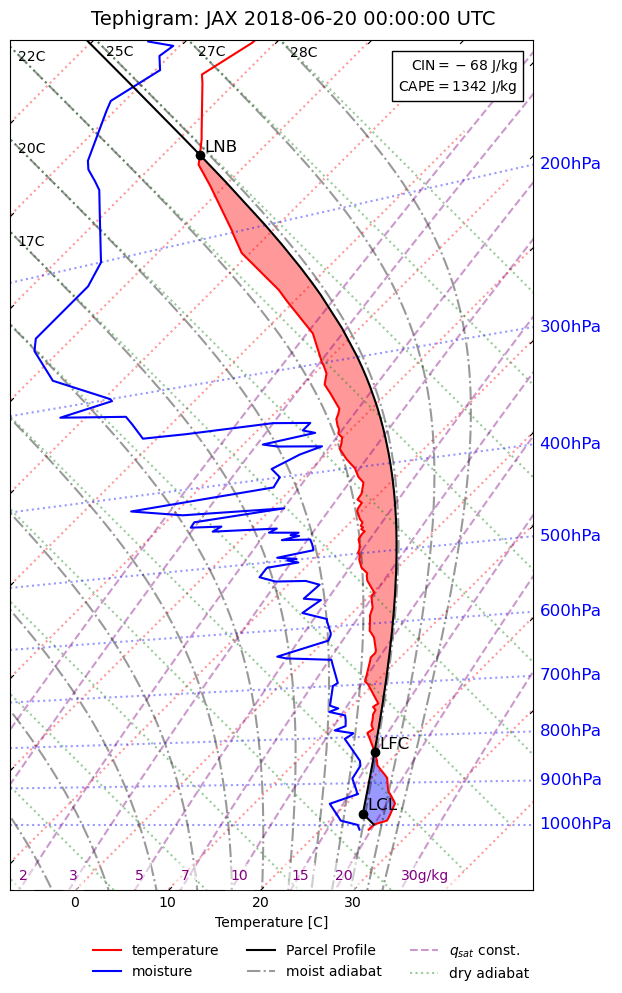
\includegraphics[width=0.75\textwidth]{figures/example_tephigram.png}
    \caption[
    An illustration of parcel ascent on a tephigram for a sounding taken on 2018-06-20 00:00 \acrshort{utc} at Jacksonville, Florida
    ]{
    An illustration of parcel ascent on a tephigram for a sounding taken on 2018-06-20 00:00 \acrshort{utc} at Jacksonville, Florida. The environmental temperature profile is shown by the red line, and the dewpoint temperature by the blue line. The path of the parcel, which starts near the surface, is shown by the black line. Points marking the \acrshort{lcl}, \acrshort{lfc} and \acrshort{lnb} are shown. The \acrshort{cape} and \acrshort{cin} are shown by the red and blue areas respectively.
    }
    \label{fig:parcel_ascent}
\end{figure}

From its initial position, the parcel is assumed to undergo adiabatic cooling as it is lifted until its temperature reaches that of the dew point of the initial airmass. 
At this point, the \acrshort{lcl}, the saturation of the airmass reaches 100\%, condensation occurs and the cloud begins to form. 
Beyond this point, the temperature of the parcel is assumed to follow the moist pseudo-adiabatic lapse rate. 
As this lapse rate is less than that of an environment with conditional instability, as the parcel continues to rise it will reach a point where its temperature is greater than that of the surrounding environment referred to as the \acrshort{lfc}. 
Above the \acrshort{lfc} the parcel will experience positive buoyancy. 
As the moist adiabatic lapse rate approaches that of the dry adiabatic lapse rate at low temperature and humidity (and hence at higher altitudes), and the environmental lapse rate reduces as it approaches the tropopause layer \citep{fueglistaler_tropical_2009}, the parcel will cool below the temperature of the surrounding environment. 
The point at which the temperature profile of the parcel again crosses that of the environment is called the \acrfull{lnb}. 
Although the air parcel may continue to rise above this point due to its momentum, negative buoyancy will act to halt its ascent.

Two further properties related to convection are also shown on the tephigram. 
\acrshort{cape} can be calculated as the area between the parcel temperature profile and the environment profile between the \acrshort{lfc} and the \acrshort{lnb}, showing clearly how \acrshort{cape} is the total work exerted by positive buoyancy forces between these two levels. 
From this, \acrshort{cape} can be used to calculate the theoretical maximum updraft velocity if all \acrshort{cape} is converted to kinetic energy, although typical maximum updraft velocities are half of this amount due to the dilution of updraft plumes through mixing with the surrounding environment \citep{lemone_cumulonimbus_1980, romps_undiluted_2010}. 
Similarly, \acrfull{cin} can be calculated as the area between the temperature profiles between the initial parcel location and the \acrshort{lfc}. 
\acrshort{cin} measures the work required to lift the parcel, overcoming negative buoyancy forces, in order to reach the \acrshort{lfc}.

There are a number of caveats with the parcel approach for deep convection that must be considered. 
The convective profile of a parcel depends upon its starting conditions including initial height, temperature and humidity. 
As a result, for even a single atmospheric column, a whole ensemble of parcels initialised at different locations within the PBL can be considered, each with different values of \acrshort{lcl}, \acrshort{lfc}, \acrshort{lnb}, \acrshort{cape} and \acrshort{cin}. 
To account for this, the mixed-layer \acrshort{cape} is often calculated from the average for parcels initiated in the \acrshort{pbl} \citep{stevens_atmospheric_2005}. 
In addition, the properties of the most unstable parcel may also be found in the same manner, which may provide useful information for predicting convective initiation.

Secondly, it is generally assumed that above the \acrshort{lcl} the parcel follows the moist pseudo-adiabat, which approximates that all condensed water is removed from the parcel immediately via precipitation \citep{emanuel_atmospheric_1994}. 
Although this approximation may seem to agree with the high precipitation rates of \acrshort{dcc}s, observed profiles of convective updrafts more closely match the moist adiabatic lapse rate (which assumes that all condensed water remains within the parcel) \citep{xu_is_1989}. 
In addition, while it is often considered that MSE is conserved in convective processes this is only correct in the case of environments in hydrostatic balance \citep{peters_evaluating_2021}. 
In deep convection, where this is not the case, it is a better approximation that MSE minus \acrshort{cape} is conserved \citep{romps_mse_2015}.

Finally, and arguably most importantly, is that the parcel model assumes that there is no mixing between the air parcel and the surrounding environment, a state that is referred to as undiluted. 
In the dynamic and turbulent environment of deep convection mixing does occur, however, and it is very rare for an undiluted state to occur \citep{zipser_cumulonimbus_1980, romps_undiluted_2010}. 
The entrainment of dry air into convective updrafts due to mixing reduces both \acrshort{cape} \citep{zhang_effects_2009} and the \acrshort{lnb} \citep{masunaga_convective_2016} as it adjusts the parcel profile closer to the background temperature profile, reducing the buoyancy forces. 
Observations of \acrshort{dcc}s have shown that while the highest cloud tops of \acrshort{dcc}s reach or even exceed the \acrshort{lnb}, the majority of the anvil cloud is detrained at a level substantially below the \acrshort{lnb} \citep{takahashi_where_2012, takahashi_level_2017}.

An additional factor not considered by the parcel model is the impact of circulation on instability.
Low-level convergence may transport additional heat and moisture to the base of the profile, increasing the potential for convection.
Wind shear---change in the speed and/or direction of wind with height---may also increase instability by transporting a colder airmass over a warmer boundary layer.
Wind shear plays an important role in the behaviour of \acrshort{dcc}s which will be explored in the following section.


\subsection{Lifecycle and structure of \acrshort{dcc}s}

The lifecycle of deep convection begins with the development of instability throughout the troposphere. 
The primary driver of instability is cooling through \acrshort{lw} emissions from water vapour, which cools the troposphere at around 2\,\unit{K} per day \citep{mapes_water_2001, jeevanjee_simple_2020}. 
\acrshort{sw} heating also affects instability which leads to diurnal differences which show large land--sea contrasts. 
Over land, \acrshort{sw} absorption warms the surface during the daytime, which sensible heating transfers to the lower troposphere. 
This \acrshort{sw} heating leads to an increase in \acrshort{cape} throughout the day, and, in particular, a peak in convective initiation in the afternoon due to surface heating and the resulting enthalpy flux into the \acrshort{pbl} \citep{hendon_diurnal_1993}.
On the contrary, over the ocean, \acrshort{sw} heating has less of an effect on the surface due to the greater heat capacity of water and the ocean mixed layer. 
Instead, a peak in instability is seen during the night and early morning \citep{gray_diurnal_1977}, which is believed to be due to the effects of \acrshort{sw} heating on the mid and upper troposphere during the day \citep{wall_life_2018}. 
The diurnal cycle of convection is much less pronounced over the ocean than over land \citep{soden_diurnal_2000}.
Instability can also be driven by the relative motion of air masses. 
Over the great plains of North America, warm, moist air is transported northward from the Gulf of Mexico which leads to instability as it moves under colder air \citep{walters_airflow_2001}.

Once sufficient instability has built up throughout the troposphere for deep convection to occur, a lifting action or buoyancy perturbation must occur to overcome \acrshort{cin} and initiate the formation of a \acrshort{dcc}.
This initiating process is referred to as the `triggering' of convection.
Triggering can occur through perturbations of the first three terms in the buoyancy equation (eq.~\ref{eq:full_bouyancy}).
\acrshort{sw} heating of the surface can cause an increase in surface air temperature through sensible heat fluxes, leading to dry convection and convective initiation.
Surface heating also causes latent heat fluxes, increasing the enthalpy and moisture content of the boundary layer.
In addition, the convergence of air masses within the boundary layer can also increase buoyancy by convergences of moisture and positive pressure perturbations.
A number of mechanical lifting mechanisms are also involved in the initiation of convection.
Orographic lifting can occur when warm, moist air is blown towards mountains and cools as it ascends \citep{hodges_distribution_1997}. 
Gust fronts of cold, dense air may also act to lift warmer, moist air masses above them. 
These gust fronts may be caused by a number of processes, including synoptic frontal systems \citep{wilson_initiation_1986, jirak_observational_2007}, sea breeze \citep{tripoli_numerical_1979, park_environmental_2020}, and cold pools caused by precipitation \citep{grant_cold_2016}.

The occurrence of cumulus and cumulus congestus clouds (convective clouds in the low- and mid-troposphere \citep{johnson_trimodal_1999}) may also lead to deep convection. 
These lower-level convective clouds cause convergences of warm, moist air near the surface, building instability, and may also act to `condition’ the lower troposphere to convection by adjusting the environmental temperature profile closer to that of an ascending air parcel and hence reducing \acrshort{cin} \citep{masunaga_mechanism_2014, schulz_observing_2018}.

\begin{figure}[tp]
    \centering
    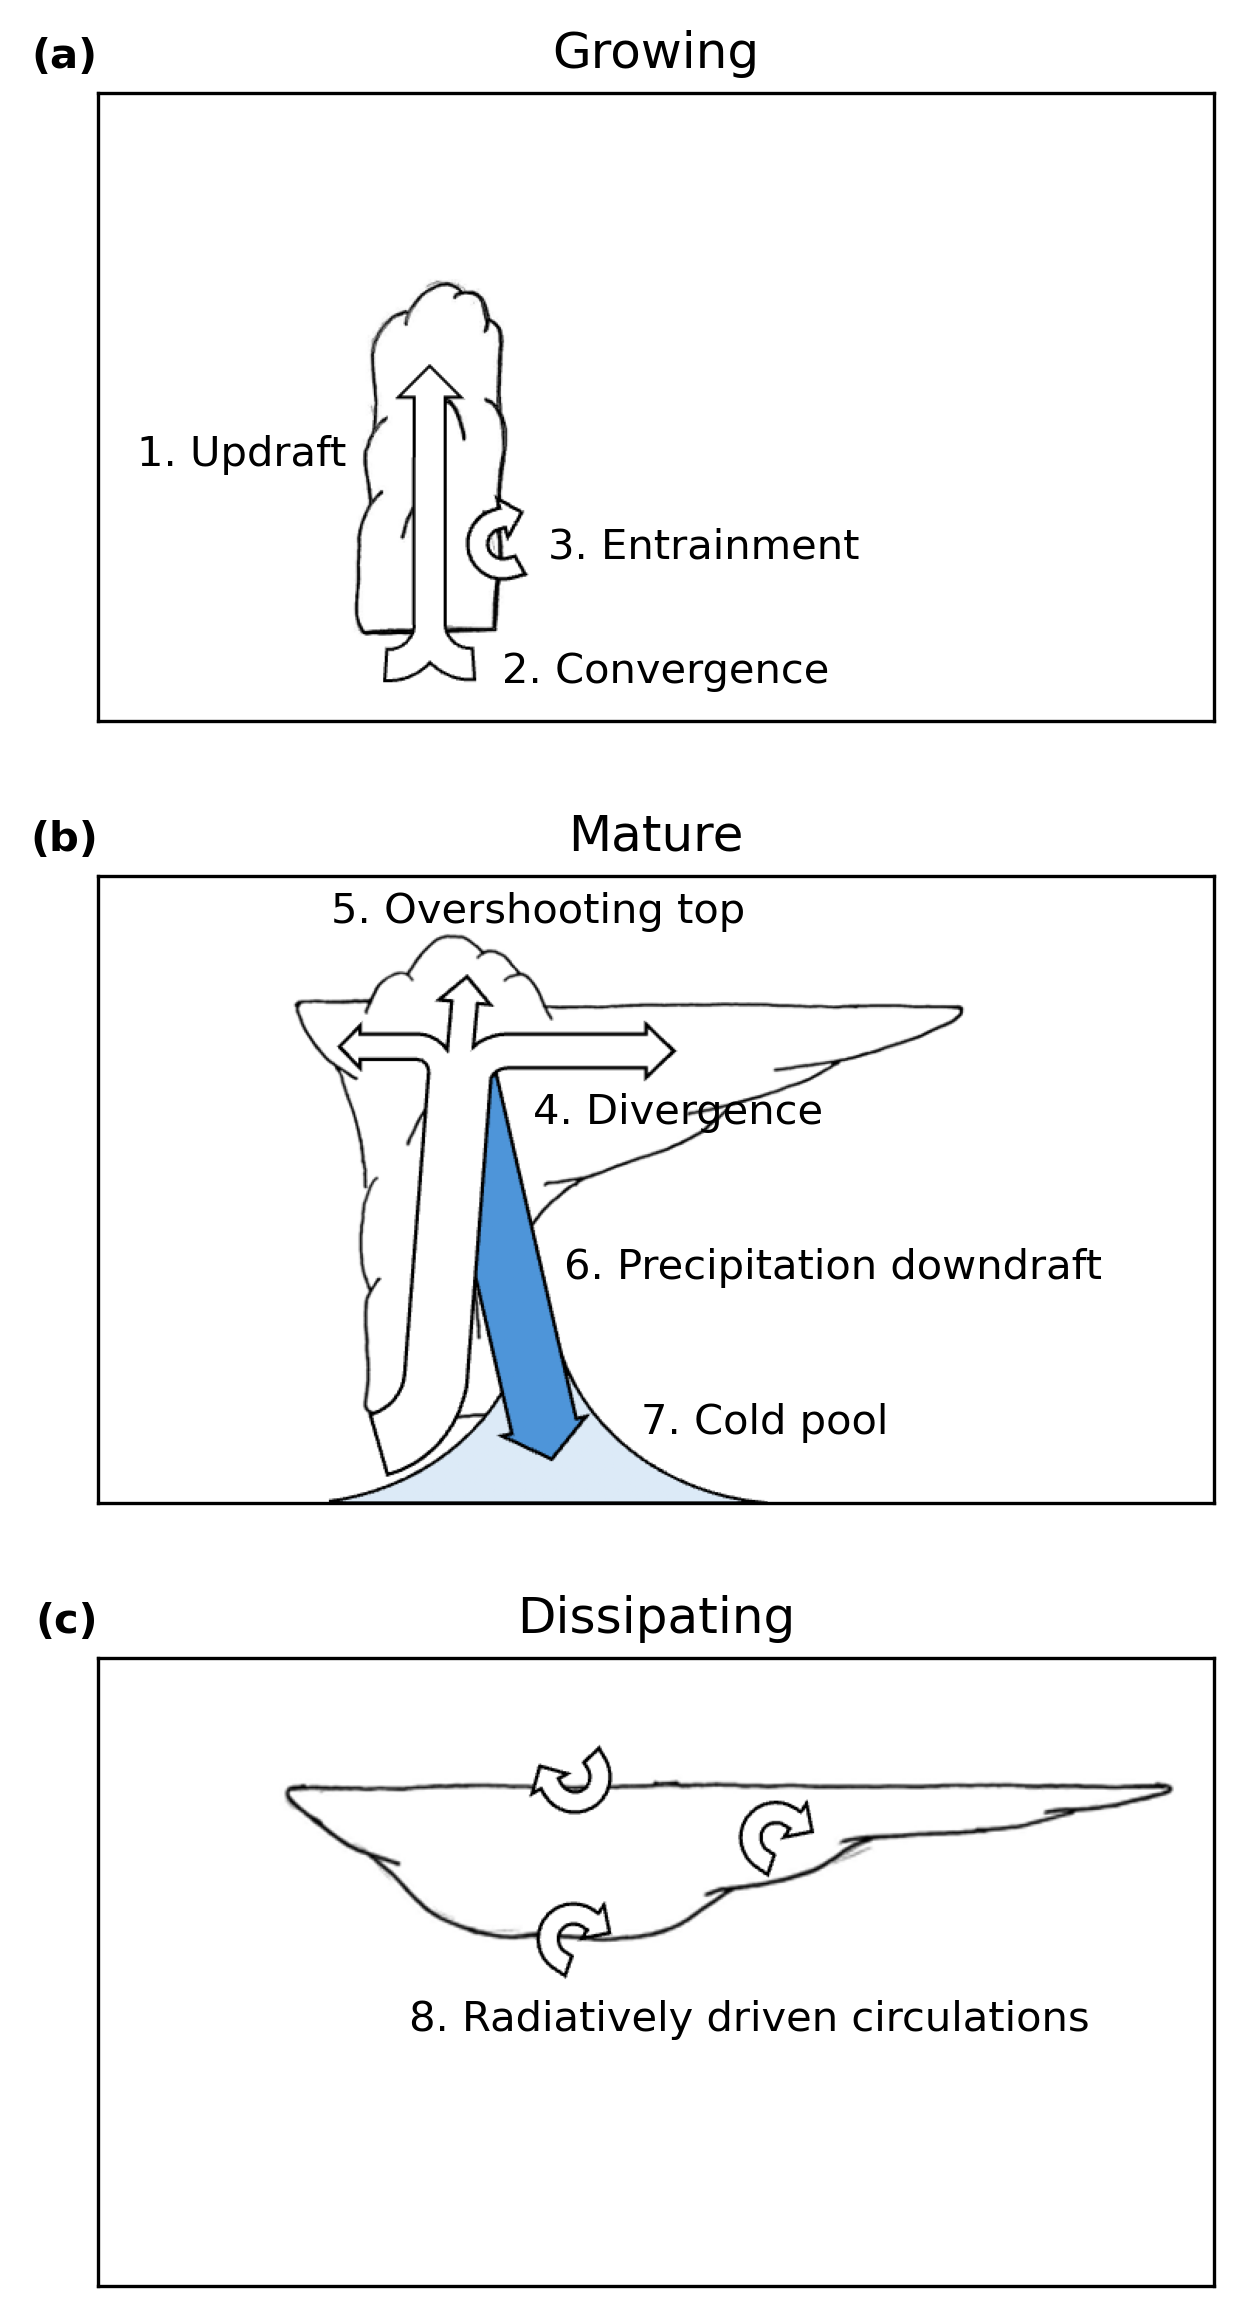
\includegraphics[width=0.5\textwidth]{figures/Intro_DCC_lifecycle.png}
    \caption[
    An illustration of the three lifecycle phases of an isolated \acrshort{dcc}
    ]{
    An illustration of the three lifecycle phases of an isolated \acrshort{dcc}: the growing (a), mature (b) and dissipating (c) phases. In the growing phase the formation of a convective updraft (1) through positive buoyancy and convergence of warm, moist air at the cloud base (2) lead to a convective core that rapidly increases in. Turbulent mixing with the surrounding environment (3) dilutes the updraft, reducing the buoyancy and hence vertical velocity. In the mature phase, the updraft reaches its \acrshort{lnb} resulting in divergence (4) and the formation of an anvil cloud. The momentum of the updraft within the core may result in it reaching the stratosphere, leading to an overshooting top (5). The onset of precipitation leads to downdrafts (6) due to hydrometeor drag and evaporative cooling, compensation for the downdraft. At the surface, this causes cold pools (7) which disrupt the inflow of air to the base of the storm, preventing further convective activity. In the dissipating phase there are no more convective dynamics, but radiative driven circulations (8) act to thin the thicker anvils due to entrainment of surrounding, dry air, but increase the lifetime of thinner anvils.
    }
    \label{fig:dcc_lifecycle_illustration}
\end{figure}

Once initiated, the lifecycle of \acrshort{dcc}s can be separated into three sections: a growing phase, where the core develops vertically (fig.~\ref{fig:dcc_lifecycle_illustration}\,a); a mature phase in which the anvil cloud develops horizontally while convection continues within the core (fig.~\ref{fig:dcc_lifecycle_illustration}\,b); and a dissipating phase in which the anvil cloud dissipates after convective activity ceases within the core (fig.~\ref{fig:dcc_lifecycle_illustration}\,c) \citep{wall_life_2018}.
For isolated \acrshort{dcc}s (those consisting of a single core) the overall lifecycle typically spans 1-3~hours \citep{chen_diurnal_1997}.
However, \acrshort{dcc}s may also form with multiple cores feeding a single anvil cloud \citep{roca_simple_2017}, and in these cases may span areas several orders of magnitude larger \citep{houze_mesoscale_2004}, and exist for 10-20~hours or longer \citep{chen_diurnal_1997}.

The initiation stage occurs between the point of initiation and the time at which the top of the convective core stops growing upwards.
During this stage precipitation may occur in both the warm and ice phases, and the horizontal growth of the cloud is small in comparison to the vertical growth.
The initiation stage can be further broken down into the periods before and after the onset of freezing.
Freezing releases additional latent heat of fusion, however this may not contribute additional buoyancy as it is compensated for by the environment \citep{seeley_tropical_2016}.

Due to the large vertical velocities and high supersaturation present in deep convective updrafts, freezing is dominated by homogeneous freezing processes.
Furthermore, the intense dynamics result in a high rate of secondary ice production through the collision of droplets and rime--splintering.
As a result, \acrshort{dcc}s tend to form with a large number of small ice particles.
In convective updrafts with large vertical velocity, the momentum of the growing cloud may propel it above the \acrshort{lnb}.
This produces a phenomenon known as an overshooting top.
As the cloud will continue to cool adiabatically as they rise, the tops of these updrafts can reach substantially colder temperatures than the surrounding environment \citep{proud_recordlow_2021}.

The mature stage occurs after the top of the \acrshort{dcc} has reached the level of neutral buoyancy.
The heaviest rates of convective precipitation occur during this stage, and the anvil cloud is formed \citep{houze_chapter_2014}.
The occurrence of heavy precipitation suppresses the convective core both through the generation of downdrafts and through the stabilisation effect of evaporating rain droplets.
This process will eventually weaken and dissipate the convective core of the \acrshort{dcc} unless the wind shear is large enough to advect the convective rainfall away from the convective core.
Furthermore, the evaporation of falling precipitation leads to the divergence of cold, dense air near the surface.
These cold pools may suppress further convective activity, while their gust fronts can also trigger new convective initiations.

The final stage of the \acrshort{dcc} lifecycle occurs after the convective core has dissipated and convective rainfall has stopped, and is referred to as the dissipating phase.
During this phase, the anvil cloud may continue to expand, with maximum anvil cloud extent occurring much later than maximum convective intensity \citep{futyan_deep_2007}.
Additional, stratiform, precipitation may occur throughout the anvil cloud, but this will not be as intense as the earlier convective precipitation \citep{houze_chapter_2014}.
The dissipating stage may also be split into two separate periods; those before and after the end of stratiform precipitation \citep{wall_life_2018}.

\acrshort{dcc}s can also be categorised spatially into three components.
Firstly, the core region, in which the convective updraught and convective precipitation occur.
Secondly, the anvil or cloud shield, which consists of a large area of thick cloud surrounding the core at the level of neutral buoyancy, and within which stratiform precipitation may occur.
Finally, the area of cirrus outflow, where thin ice cloud extends beyond the edge of the anvil cloud, particularly within the dissipating phase \citep{lilly_cirrus_1988}.
This structure of an isolated \acrshort{dcc} is also referred to as a `hot tower' \citep{riehl_northeast_1951}.

Radiative heating of the anvil cloud base and cooling of the anvil cloud top causes two regions of instability to occur. 
These unstable profiles drive circulations at the cloud base and top which increase the entrainment of dry air into the anvil while also lifting the anvil higher in the troposphere. 
While SW heating during the daytime reduces the instability at the cloud top, the greater LW heating at the cloud base results in a greater net dissipation of anvil during the daytime \citep{sokol_tropical_2020}. 
As the anvil cloud thins, these two regions of instability join into a single lapse rate. 
This state drives circulations within the anvil cloud which lift ice particles, reducing sedimentation and increasing particle growth \citep{gasparini_opinion_2023}. 
These circulations prolong the lifetime of the thin anvil cloud \citep{sokol_tropical_2020}. 
Further thinning of the cirrus anvil results in uniform radiative heating throughout the anvil, ending the circulation and leading the to complete dissipation of the anvil cloud. 


\subsection{Convective organisation}

While the majority of \acrshort{dcc}s form as isolated storms, with a single convective core that detrains its own anvil cloud \citep{riehl_northeast_1951}.
In other cases, \acrshort{dcc}s exist with multiple convective cores feeding a single anvil cloud \citep{zipser_role_1969, nakazawa_tropical_1988}.
At the largest end of this progression are \acrfullpl{mcs}, which occur when a cluster of deep convective cores form a single large area of anvil referred to as a cloud shield \citep{roca_simple_2017}.
These \acrshort{mcs} cloud shields can cover an area of greater than 10,000~km\textsuperscript{2}, several orders of magnitude greater than that of individual \acrshort{dcc}s \citep{houze_mesoscale_2004}.

The convective cores that form \acrshort{mcs}s do not group together at random, but are instead clustered by a complex group of processes that are referred to as convective organisation.
In general, these processes tend to lead to the triggering of new convective cores that feed the same cloud shield, expanding and extending the life of the system as they do.
\acrshort{mcs}s occur in a number of shapes and sizes, including mesoscale convective complexes, squall lines and tropical cloud clusters \citep{tsakraklides_global_2003a} which each have their own unique properties.
However, all \acrshort{mcs}s display large-scale processes that initiate new cores, and increase the size and lifetime of the anvil

The lifecycle of \acrshort{mcs}s can be described similarly to that of isolated \acrshort{dcc}s through the three-phase growing, mature, dissipating structure \citep{futyan_deep_2007}.
It should be kept in mind however that when applied to \acrshort{mcs}s, these lifecycle stages do not represent the changes in convective processes as described for isolated \acrshort{dcc}s, but the mesoscale development and decay of the entire system.
The lifetime of these systems is substantially lengthened, with typical \acrshort{mcs}s lasting for 10 to 20 hours or longer \citep{chen_diurnal_1997}.
In particular, there is an increase in the lengths of the initiation and mature phases compared to isolated \acrshort{dcc}s \citep{wall_life_2018} due to the continuous development of new cores throughout the active lifetime of the \acrshort{mcs}.
The total lifetime of \acrshort{mcs}s is determined by the rate at which new cores are triggered, and observations have shown that they tend to decay once the area of convective cores falls below 10\% of the total anvil area \citep{elsaesser_simple_2022}.

A key feature that distinguishes \acrshort{mcs}s from smaller \acrshort{dcc}s is the development of large, mesoscale circulations that occur on larger scales than that of individual convective cores.
As well as the convergence of heat and moisture at low levels due to the convective cores, this mesoscale circulation draws in additional air from the surrounding areas at the mid-levels of the atmosphere.
This mid-level air does enter the cloud shield through the convective cores, but instead condenses at higher altitudes, leading to a top-heavy latent heating profile within the cloud shield \citep{schumacher_tropical_2004}.
These organised convective cloud systems have thermodynamic impacts on the environment to a much greater extent than isolated \acrshort{dcc}s.
The large cloud shields of the \acrshort{mcs} s result in much larger amounts of stratiform precipitation than individual \acrshort{dcc}s, which is distributed over a much wider area \citep{houze_chapter_2014}.
These organised convective cloud systems have thermodynamic impacts on the environment to a much greater extent than isolated \acrshort{dcc}s, with idealised simulations showing that the thermodynamic interactions of organised convective systems can propagate thousands of kilometres within the troposphere \citep{beucler_budget_2019}.
Over time, the mesoscale circulation results in a moistening of the convective system and a drying of the surrounding atmosphere, creating a sharp contrast between the two regions \citep{bretherton_energybalance_2005}.

\acrshort{mcs}s are also characterised by both high rates and large volumes of precipitation, providing the majority of precipitation throughout the tropics as well as in many other regions \citep{feng_global_2021}.
Unlike isolated \acrshort{dcc}s, much of the precipitation occurs not as convective rainfall, but as stratiform rain from the cloud shield \citep{schumacher_stratiform_2003}.
As much as 70\,\% of the total precipitation of an \acrshort{mcs} can come from the stratiform rain, with a higher proportion observed over the ocean than in \acrshort{mcs}s over land.
Much of this stratiform precipitation can be attributed to the mid-level, mesoscale inflow to the cloud shield as well as the top-heavy latent heating profile.

The processes through which \acrshort{mcs}s form in the first place are still uncertain, however \citep{houze_100_2018}.
Convective organisation processes have been observed in satellite remote sensing, radiative-convective equilibrium models and cloud-resolving models \citep{holloway_observing_2017}. 
The formation and lifetime of \acrshort{mcs}s are strongly linked to the dynamics of the surrounding environment through the convergence of moist, low-level air and the divergence of air at the top of the \acrshort{mcs}  \citep{houze_chapter_2014}. 
Cold pools have a strong influence on the organisation of convective cores, and set the scales over which organisation occurs \citep{jeevanjee_convective_2013}, as their gust fronts, transport of moisture and collisions are vital to triggering new convection within \acrshort{mcs}s \citep{feng_mechanisms_2015}.
\acrshort{mcs}s have a tendency to trigger additional convection around the storm, blurring the boundary between the \acrshort{mcs} and isolated convection \citep{mapes_gregarious_1993}.

\acrshort{mcs}s are, in general, poorly represented in large-scale climate models due to the inability of the parameterised convection to organise between grid squares \citep{houze_100_2018}.
While convective resolving models have been proposed as a solution to this issue \citep{stevens_added_2020}, these models still do not represent \acrshort{mcs}s accurately with a tendency towards too little organisation \citep{prein_sensitivity_2021}.
Gaining a better understanding of the properties and processes of \acrshort{mcs}, both in observations and models, is vital therefore for improving their representation \citep{feng_mesoscale_2023}.
Changes in convective organisation have important effects on the global climate, with increases in organisation correlated with domain-wide \acrshort{toa} cooling in satellite observations \citep{bony_observed_2020}, and so future changes in organisation may have a large influence on the equilibrium climate sensitivity.


\section{Anvil Radiative Feedbacks} \label{sec:anvil_feedbacks}

There are a number of hypotheses regarding the \acrshort{cre} of tropical anvil clouds that consider whether the neutral \acrshort{cre} of tropical anvils is the result of a feedback mechanism. 
\citet{ramanathan_cloud-radiative_1989} proposed the thermostat hypothesis in which, in response to a warming environment, anvil clouds produce thicker cirrus which acts to cool the tropics through increased \acrshort{sw} reflectance. 
The Iris hypothesis proposes that anvil cirrus will decrease in area, resulting in greater \acrshort{lw} emission from the surrounding clear-sky regions.
\citet{lindzen_does_2001} first proposed this as a result of increased precipitation efficiency, however evidence for this effect is disputed \citep{genio_climatic_2002, lin_examination_2004}.
\citet{bony_thermodynamic_2016} proposed a `stability iris' feedback, in which the established trends of increased dry static stability \citep{held_robust_2006} and a reduction in the tropical overturning circulation \citep{vecchi_global_2007} reduce the detrainment of anvil cirrus.
Although the anvil cloud response is generally considered to be a negative climate feedback, the predicted magnitude varies widely and it represents the greatest uncertainty among all cloud feedbacks \citep{sherwood_assessment_2020}.

On the other hand, the \acrfull{fat} hypothesis argues that the anvil \acrfull{ctt} remains constant in a warming climate, and the greater difference between anvil and surface temperatures result in a positive \acrshort{lw} feedback \citep{hartmann_important_2002}.
The basis for \acrfull{fat} is that \acrshort{lw} cooling of the troposphere due to water vapour becomes inefficient below 220\,\unit{K} \citep{jeevanjee_simple_2020}, which, if relative humidity remains constant, fixes the top of the convectively active troposphere at this isotherm. 
While there is evidence that this is the case for the largest \acrshort{dcc} anvils, the increase in static stability may result in a reduced positive feedback due to a `proportionally higher' anvil temperature \citep{zelinka_why_2010} which more closely matches the \acrshort{lw} response of tropical clouds in global climate models.
While satellite observations have shown a trend in anvil cloud height \citep{norris_evidence_2016}, there is not yet sufficient evidence to distinguish this from inter-annual variability \citep{takahashi_when_2019}.
\citet{seeley_fat_2019}, argued that \acrshort{fat} is a weak constraint on anvil temperature as while the radiative tropopause temperature remains fixed, the temperature of the tropopause lapse rate inversion can vary widely. 
Furthermore, as anvils tend to detrain below the tropopause, \citep{takahashi_level_2017, wang_observational_2020}, anvil temperature and the tropopause temperature may only be weakly connected.
\citet{seidel_temperatures_2022} however found the inclusion of CO\textsubscript{2} radiative heating produces anvil temperatures consistent with \acrshort{fat}.

While the iris and \acrshort{fat} feedbacks may act to cancel each other out, and hence maintain the neutral \acrshort{cre} of tropical anvil clouds, there are other potential feedback mechanisms that may influence this balance.
\citet{hill_climate_2023} showed recently that climate models underestimate dynamically driven cloud feedbacks.
Furthermore, convective instability is expected to scale with temperature in the same manner as the Clausius-Clapeyron relation \citep{seeley_why_2015, agard_clausius_2017}, and some observations of tropical anvil clouds have instead suggested that warming of the surface invigorates convection \citep{igel_cloudsat_2014}.
This invigoration effect may result in colder anvil \acrfull{ctt}, and hence a stronger warming feedback.
Multi-decadal satellite observations have shown a cooling of upper tropospheric cloud temperature over land \citep{liu_observed_2023}, indicating that changes in convective processes may lead to stronger cooling feedbacks.

A recent criticism of the \citet{sherwood_assessment_2020} decomposition of anvil feedbacks into the area response and the height response is that, by ignoring changes in the optical properties and structure of anvil clouds, these feedbacks are merged into the calculated iris effect, increasing its uncertainty \citep{raghuraman_observational_2024}.
\citet{mckim_weak_2024} proposed that the anvil area feedback of --0.40\,\unit{W m\textsuperscript{-2} K\textsuperscript{-1}} from \citet{sherwood_assessment_2020} would require an unrealistic anvil area change of --20\,\unit{\% K\textsuperscript{-1}}, indicating that there are other mechanisms contributing to the measured change in anvil \acrshort{cre}.
Recent work has proposed that the anvil cloud response reduces the area of thicker anvils with high \acrshort{iwc}, but not thinner cirrus, resulting in a much smaller overall feedback \citep{mckim_weak_2024, sokol_greater_2024}.

Changes to the lifecycle and diurnal cycle of deep convection may also be an important factor, particularly when considering the \acrshort{sw} feedback. 
\citet{nowicki_observations_2004} used estimates of \acrfull{toa} \acrshort{lw} and \acrshort{sw} radiative fluxes from \acrfull{seviri} observations to estimate the diurnal cycle of anvil \acrshort{cre} over equatorial Africa and the equatorial Atlantic. 
They found that shifting the diurnal cycle of deep convection in these regions could change the \acrshort{cre} by \textpm 10\,\unit{Wm\textsuperscript{-2}}, but did not track the properties of individual \acrshort{dcc}s.
\citet{bouniol_macrophysical_2016} compared \acrshort{cre} and cloud radiative heating rates to anvil cloud properties to investigate how radiative heating affects the anvil cloud evolution.
These observations were made with polar orbiting instruments however, and they highlighted the need for geostationary observations to characterise the evolution of individual anvil clouds.
Subsequent research used \acrshort{dcc} tracking methods to better characterise the lifecycle of observed anvil clouds \citep{bouniol_life_2021}, but as the radiative flux data was provided by polar-orbiting satellites the \acrshort{cre} could not be measured over the lifetime of the \acrshort{dcc}.


\section{Detection and tracking of deep convection} \label{sec:tracking_timeline}

The detection and tracking of clouds has been performed since the earliest sequences of remote sensing imagery from weather radar and geostationary satellites \citep{menzel_cloud_2001}.
\citet{fujita_study_1968} compared sequences of images observed by the first geostationary weather satellite to those taken using an all-sky camera, and found that by comparing subsequent observations from the satellite one could calculate \acrshort{amv}s similar to those observed on the ground.
This tracking of cloud position was performed by hand, and subsequently a plastic stencil `computer' was designed to calculate cloud velocities taking into account the satellite viewing geometry \citep{fujita_present_1969}.
While these early methods compared print-outs of satellite imagery by hand, shortly after a digital computer system was developed to show sequences of images \citep{chang_metracom_1973}.
Although detection and tracking were still performed manually (albeit with the user selecting cloud positions in subsequent images using the cursor), velocity calculation was performed automatically.
Wider adoption of this technology was applied to produce \acrshort{amv}s during field campaigns in the mid- to late-1970s \citep{tecson_cloud-motion_1975}.

There was, however, concern regarding the manual tracking of cloud velocity.
This task was both time consuming and also open to subjective judgement which made uncertainties hard to estimate.
\citet{fujita_satellite-tracked_1975} found large variations in \acrshort{amv}s produced using these methods.
Early efforts at automation applied cross-correlation techniques, previously used with weather radar, to estimate \acrshort{amv}s in geostationary satellite imagery \citep{leese_determination_1970}.
\citet{endlich_use_1971} applied a pattern matching technique to `brightness centres' in visible satellite imagery to estimate cloud motion.
\citet{rinehart_three-dimensional_1978} produced a cross-correlation algorithm for the estimation of convective cell motion in 3-D weather radar observations.
While these automated methods provided more accurate motion estimates than humans, they were less capable of detecting independent cloud motions both due to errors introduced by noise, and also due to the visible imagery provided by early geostationary satellites meaning it was difficult to distinguish clouds at different altitudes.

Automatic methods for the detection and tracking of \acrshort{dcc}s were developed for both radar reflectivity \citep{crane_automatic_1979} and geostationary satellite \acrshort{lw} \acrfull{ir} \acrfull{bt} \citep{endlich_automatic_1981}.
Both of these methods detected \acrshort{dcc} features by labelling the area surrounding local extrema (maxima for radar reflectivity, minima for \acrshort{bt}) in individual images.
The addition of 11\,\unit{\mu m} \acrshort{ir}-window \acrshort{bt} channels to the first operational \acrshort{goes} and Meteosat weather satellites allowed \acrshort{dcc}s to be distinguished from low clouds.
The centroids (the location of the feature represented as a single point) of these detected features were then linked to create \acrshort{dcc} tracks through the use of cost-minimisation algorithms with sought to find the best match between pairs of features detected at subsequent time steps.
By explicitly detecting features to track, these algorithms both improved upon the weakness of previous algorithms, but also allowed the properties of tracked objects to be studied beyond their motion vectors.

The development of \acrshort{dcc} detection and tracking algorithms continued in parallel for both radar and satellite observations.
\citet{rosenfeld_objective_1987} and \citet{williams_satellite-observed_1987} both developed overlap tracking techniques for radar reflectivity and satellite \acrshort{bt} observations respectively.
Unlike the prior centroid-based tracking methods, these overlap methods took into account the spatial extent of detected features by linking subsequent pairs of features based on those which shared the largest overlapping area.
By removing the approximation of a point-like feature, the overlap techniques better handle cases of \acrshort{dcc}s with larger, more complex shapes.
The downside to this approach, however, is that, unless the spatial extent of the \acrshort{dcc} is propagated using an estimate of the storm motion, it requires that the detected features do not move further than their diameter between subsequent observations.
As a result, for small, fast-moving objects (such as convective cells), or observations that are more widely spaced, overlap methods perform poorly.

Early detection and tracking algorithms were strongly limited by the available computational power which restricted tracking to only a small number of \acrshort{dcc}s. 
Furthermore, the accuracy of early algorithms was such that human verification of tracked objects was still required. 
The majority of algorithms were designed with only a single source of observations, which, in particular for weather radars, reduced the area over which tracking could be performed. 
While geostationary satellites provided larger areas of observations, the low spatial and temporal resolution of early sensors limited studies to only large and long-lived \acrshort{mcs}s. 
\citet{maddox_mesoscale_1980a} tracked mesoscale convective complexes over the US, and subsequent studies showed their distributions globally \citep{laing_global_1997}.

Subsequent development produced trends in both those algorithms used to track \acrshort{dcc}s in satellite imagery, and those using weather radar.
Algorithms using geostationary satellite imagery focused on the study of \acrshort{mcs}s, and tended to use overlap-based tracking methods \citep{arnaud_automatic_1992, evans_procedure_1996, carvalho_satellite_2001, morel_climatology_2002}.
On the other hand, tracking algorithms using radar reflectivity tended to focus on the tracking of convective cells, and favoured centroid-based tracking approaches \citep{dixon_titan_1993, johnson_storm_1998, handwerker_cell_2002}.
Across both sets of algorithms, the use of fixed thresholds rather than extrema for locating features became favoured both due to the low computational cost, ease of customisation and resilience to noise \citep{augustine_mesoscale_1988}.
While the majority of approaches used a single threshold, a number of algorithms introduced the use of multiple thresholds to better characterise the detected features of \acrshort{dcc}s.
\citet{johnson_storm_1998} used a sequence of increasingly larger thresholds to better distinguish individual convective cells, and classify them according the intensity.
For \acrshort{mcs} detection, the `detect-and-spread' approach was used by \citet{evans_procedure_1996} and \citet{boer_lagrangian_1997} to better measure the area of \acrshort{mcs}s by first detecting the `core' using a cold \acrshort{bt} threshold and then detecting the surrounding cloud area using a warmer threshold.
It should be noted however that \citet{augustine_mesoscale_1988} argued that the area estimated using the warmer threshold is highly subjective.

\citet{hodges_general_1994} developed a more general algorithm for use with multiple gridded datasets, including model data, and subsequently expanded this approach to consider detection and tracking on a sphere for use with \acrshort{gcm}s \citep{hodges_feature_1995}.
The low spatial and temporal resolution of \acrshort{gcm}s of the time however meant that detection and tracking of individual \acrshort{dcc}s was not possible.
Other data, such as rainfall measurements and lightning flash observations, were also used to develop detection and tracking algorithms \citep{steinacker_automatic_2000}, however the vast majority of algorithms continued to use either radar reflectivity or geostationary satellite \acrshort{bt} observations.

The development of radar detection and tracking algorithms was strongly driven by the needs for nowcasting (short-term, 30- to 60-minute forecasts) of convective activity \citep{wilson_nowcasting_1998}.
As these algorithms are required to predict the future motion of observed \acrshort{dcc}s, good estimates of the storm motion, including growth and decay, are required.
Development of these algorithms, therefore, focused primarily on the tracking aspect rather than the detection of \acrshort{dcc}s \citep{lakshmanan_objective_2010}.
The Sydney 2000 Olympics provided both a demonstration of, and comparison between, the capabilities of multiple tracking algorithms \citep{keenan_sydney_2003}.
The study into the performance of these algorithms found that no particular tracking approach worked best overall, and that each had strengths and weaknesses in different situations \citep{wilson_sydney_2004}.
In response, subsequent algorithms used hybrid approaches which combined multiple tracking methods to provide better performance over a range of scenarios \citep{lakshmanan_warning_2007, han_3d_2009}.

The second generation of geostationary weather satellites provided greater capability to track individual \acrshort{dcc}s due to both their higher spatial and temporal resolutions and increased number of channels across the visible and \acrshort{ir} spectrum.
\citet{roberts_nowcasting_2003} showed that these observations could be use to detect initiating \acrshort{dcc}s up to 30 minutes before they appear in weather radar observations.
Because of their use of a single \acrshort{bt} threshold, existing methods could only track \acrshort{dcc}s once they had matured.
While this was generally acceptable for tracking \acrshort{mcs}s, this limited their capability for tracking isolated \acrshort{dcc}s.
\citet{mecikalski_forecasting_2006} developed an algorithm which combined visible imagery, estimates of \acrshort{bt} cooling rate over multiple observations and \acrshort{amv}s to indicate convective initiation.
\citet{zinner_cb-tram_2008} used multiple \acrshort{ir} \acrshort{bt} channels from the Meteosat \acrshort{seviri} imager, along with the high resolution visible channel and motion vectors derived using a pyramidal matching algorithm to detect and track developing \acrshort{dcc}s over multiple stages from initiation to maturity.

A common theme throughout all the algorithms described so far is the separation of feature detection and tracking into separate procedures, with features detected independently at each time step.
While this allows for simplification of the overall process, the independent detection of features at each time step introduces a large degree of inconsistency in the area and location of features detected over time.
Furthermore, when using a fixed threshold, this also prevents the detection of features before or after they reach the threshold, limiting the detection of growing or decaying \acrshort{dcc}s.
A number of recent algorithms have sought to address this by combining both feature detection and tracking into a single process.
\citet{fiolleau_algorithm_2013} applied the `detect-and-spread' approach to a `3-D' stack of images over time.
By first detecting the core region using a cold \acrshort{bt} threshold, and then detecting the surrounding cloud volume using a warmer threshold, the algorithm is better able to detect the growing and decaying phases of \acrshort{dcc}s without erroneously detecting warmer clouds.
However, the algorithm does not consider the motion of the tracked objects in any manner, and so is only suitable for detecting \acrshort{mcs}s whose areas are large compared to the distance moved between observations.
\citet{thomas_data_2010} used a variational-data-assimilation model to both detect and track \acrshort{dcc}s in geostationary satellite images.
This approach not only allowed detection and tracking in a single step, but was also resilient to cases of noisy or missing data.

Improvements in climate modelling have led to new applications of cloud detection and tracking algorithms in cloud-resolving models \citep{plant_statistical_2009}, large eddy simulations \citep{dawe_statistical_2012a, heus_automated_2013} and for the evaluation of  \acrshort{gcm}s \citep{clark_application_2014}.
A wide range of modern algorithms have been developed specifically for general application to radar, satellite and model data \citep{heikenfeld_tobac_2019, ullrich_tempestextremes_2017, ullrich_tempestextremes_2021, raut_adaptive_2021, feng_pyflextrkr_2023}.
These new methods have allowed studies into the differences in \acrshort{dcc}s between observations and models, as well as the response of \acrshort{dcc}s to perturbations across multiple models \citep{marinescu_impacts_2021, feng_mesoscale_2023}.
Furthermore, the flexibility of these general purpose approaches has allowed their application for the detection and tracking of atmospheric phenomena beyond \acrshort{dcc}s \citep{bukowski_direct_2021, zhang_spaceborne_2023}.

A further focus of modern algorithm development has been for studying trends in the behaviour of \acrshort{dcc}s observed in long time series of observations, with techniques optimised to these problems \citep{ocasio_tracking_2020, hayden_properties_2021}.
Overall, these developments have allowed cloud tracking studies to move from smaller cases to large data problems involving the properties of tens, if not hundreds of thousands of \acrshort{dcc}s.

\acrshort{dcc} detection and algorithms have made vast advances since the earliest approaches that supplanted human tracking.
Through this development process, the requirements for a successful algorithm have become apparent.
The detection process needs to accurately distinguish between \acrshort{dcc}s and other clouds, while also detecting the largest possible extent and proportion of the \acrshort{dcc} lifetime, while being consistent between time steps and resilient to noise.
The first two aspects pose a challenge, as in general improving one of these sensitivities means worsening the other.
The tracking approach needs to then accurately connect these features without mistakenly connecting or failing to track storms, taking into account the motion of each \acrshort{dcc} as well as splits and merges.
Many modern algorithm developments have only focused on addressing a few of these concerns, without taking into account developments made by other algorithms.
Many of the same issues from older algorithms still exist.
For example, many modern detection approaches using satellite \acrshort{bt} only use a single 11\,\unit{\mu m} channel, despite the availability of many different channels providing additional information about \acrshort{dcc} properties from modern imagers.

One of the key remaining challenges is the split in algorithms designed to track \acrshort{mcs}s and those designed to track individual \acrshort{dcc}s.
The gap in capabilities between these two approaches makes it challenging, if not impossible, to study the behaviour of \acrshort{dcc}s across a wide range of scales.
Investigating these properties, therefore, will require further developments on top of those already made on \acrshort{dcc} detection and tracking.


\section{Structure of the thesis}

Improving our knowledge of the processes influencing \acrshort{dcc}s is vital to better understanding of their response to a warming world.
Recent research has highlighted the need to study the optical properties and structure of \acrshort{dcc}s, and improve the connections between convective processes and anvil properties \citep{gasparini_opinion_2023}.
In addition, understanding how these properties change over the evolution of the anvil clouds has become an increasing focus of studies \citep{sokol_tropical_2020, wall_life_2018, bouniol_life_2021}.
The body of this thesis consists of four major chapters, through which we aim to answer several questions about the study and behaviour of \acrshort{dcc}s.
In chapter~\ref{chp:tracking_method}, a novel method for tracking both the developing cores and anvils of \acrshort{dcc}s is developed, addressing some of the limitations of existing tracking methods for the study of \acrshort{dcc}s across their entire lifecycle.
This methodology is then applied to five years of geostationary satellite observations to create a dataset linking \acrshort{dcc} properties, which is presented and analysed in chapter~\ref{chp:lifecycle}.
Further insights into the impact of convective processes on anvil clouds can be gained using this dataset.
In chapter~\ref{chp:anvil_structure}, the response of anvil cloud structure to changes in convective intensity and organisation is studied, including changes across the observed lifetime of \acrshort{dcc}.
In chapter~\ref{chp:radiative_effect} we investigate the \acrshort{cre} of individual \acrshort{dcc}s, how organisation impacts anvil \acrshort{cre} and how the effect of the observed population of \acrshort{dcc}s produces the near--zero net \acrshort{cre} seen in previous studies.

Through exploring these topics, we aim to address gaps in the observational study of \acrshort{dcc}s.
While we cannot hope to ``solve'' the response of \acrshort{dcc}s to warming, by answering these questions we can provide novel, key insights into poorly understood convective processes and their importance for climate change.
